\part{四点共圆}
\section{判定方法}
\begin{proposition}[四点共圆判定方法]
    四边形ABCD顶点均在圆O上,等价于下列任一条件成立。

    (1) A、B、C、D到同一点O的距离相同。

    (2) 存在一组对角互补。

    (3) 有一边与另两点构成的顶角度数相同。

    (4) 对角线交于F点,$AF\cdot FC = BF\cdot FD$。

    (5) 有一组对边AB、CD的延长线相交于E,若$EA\cdot EB = ED\cdot EC$。
\end{proposition}
\begin{figure}[H]
    \centering
    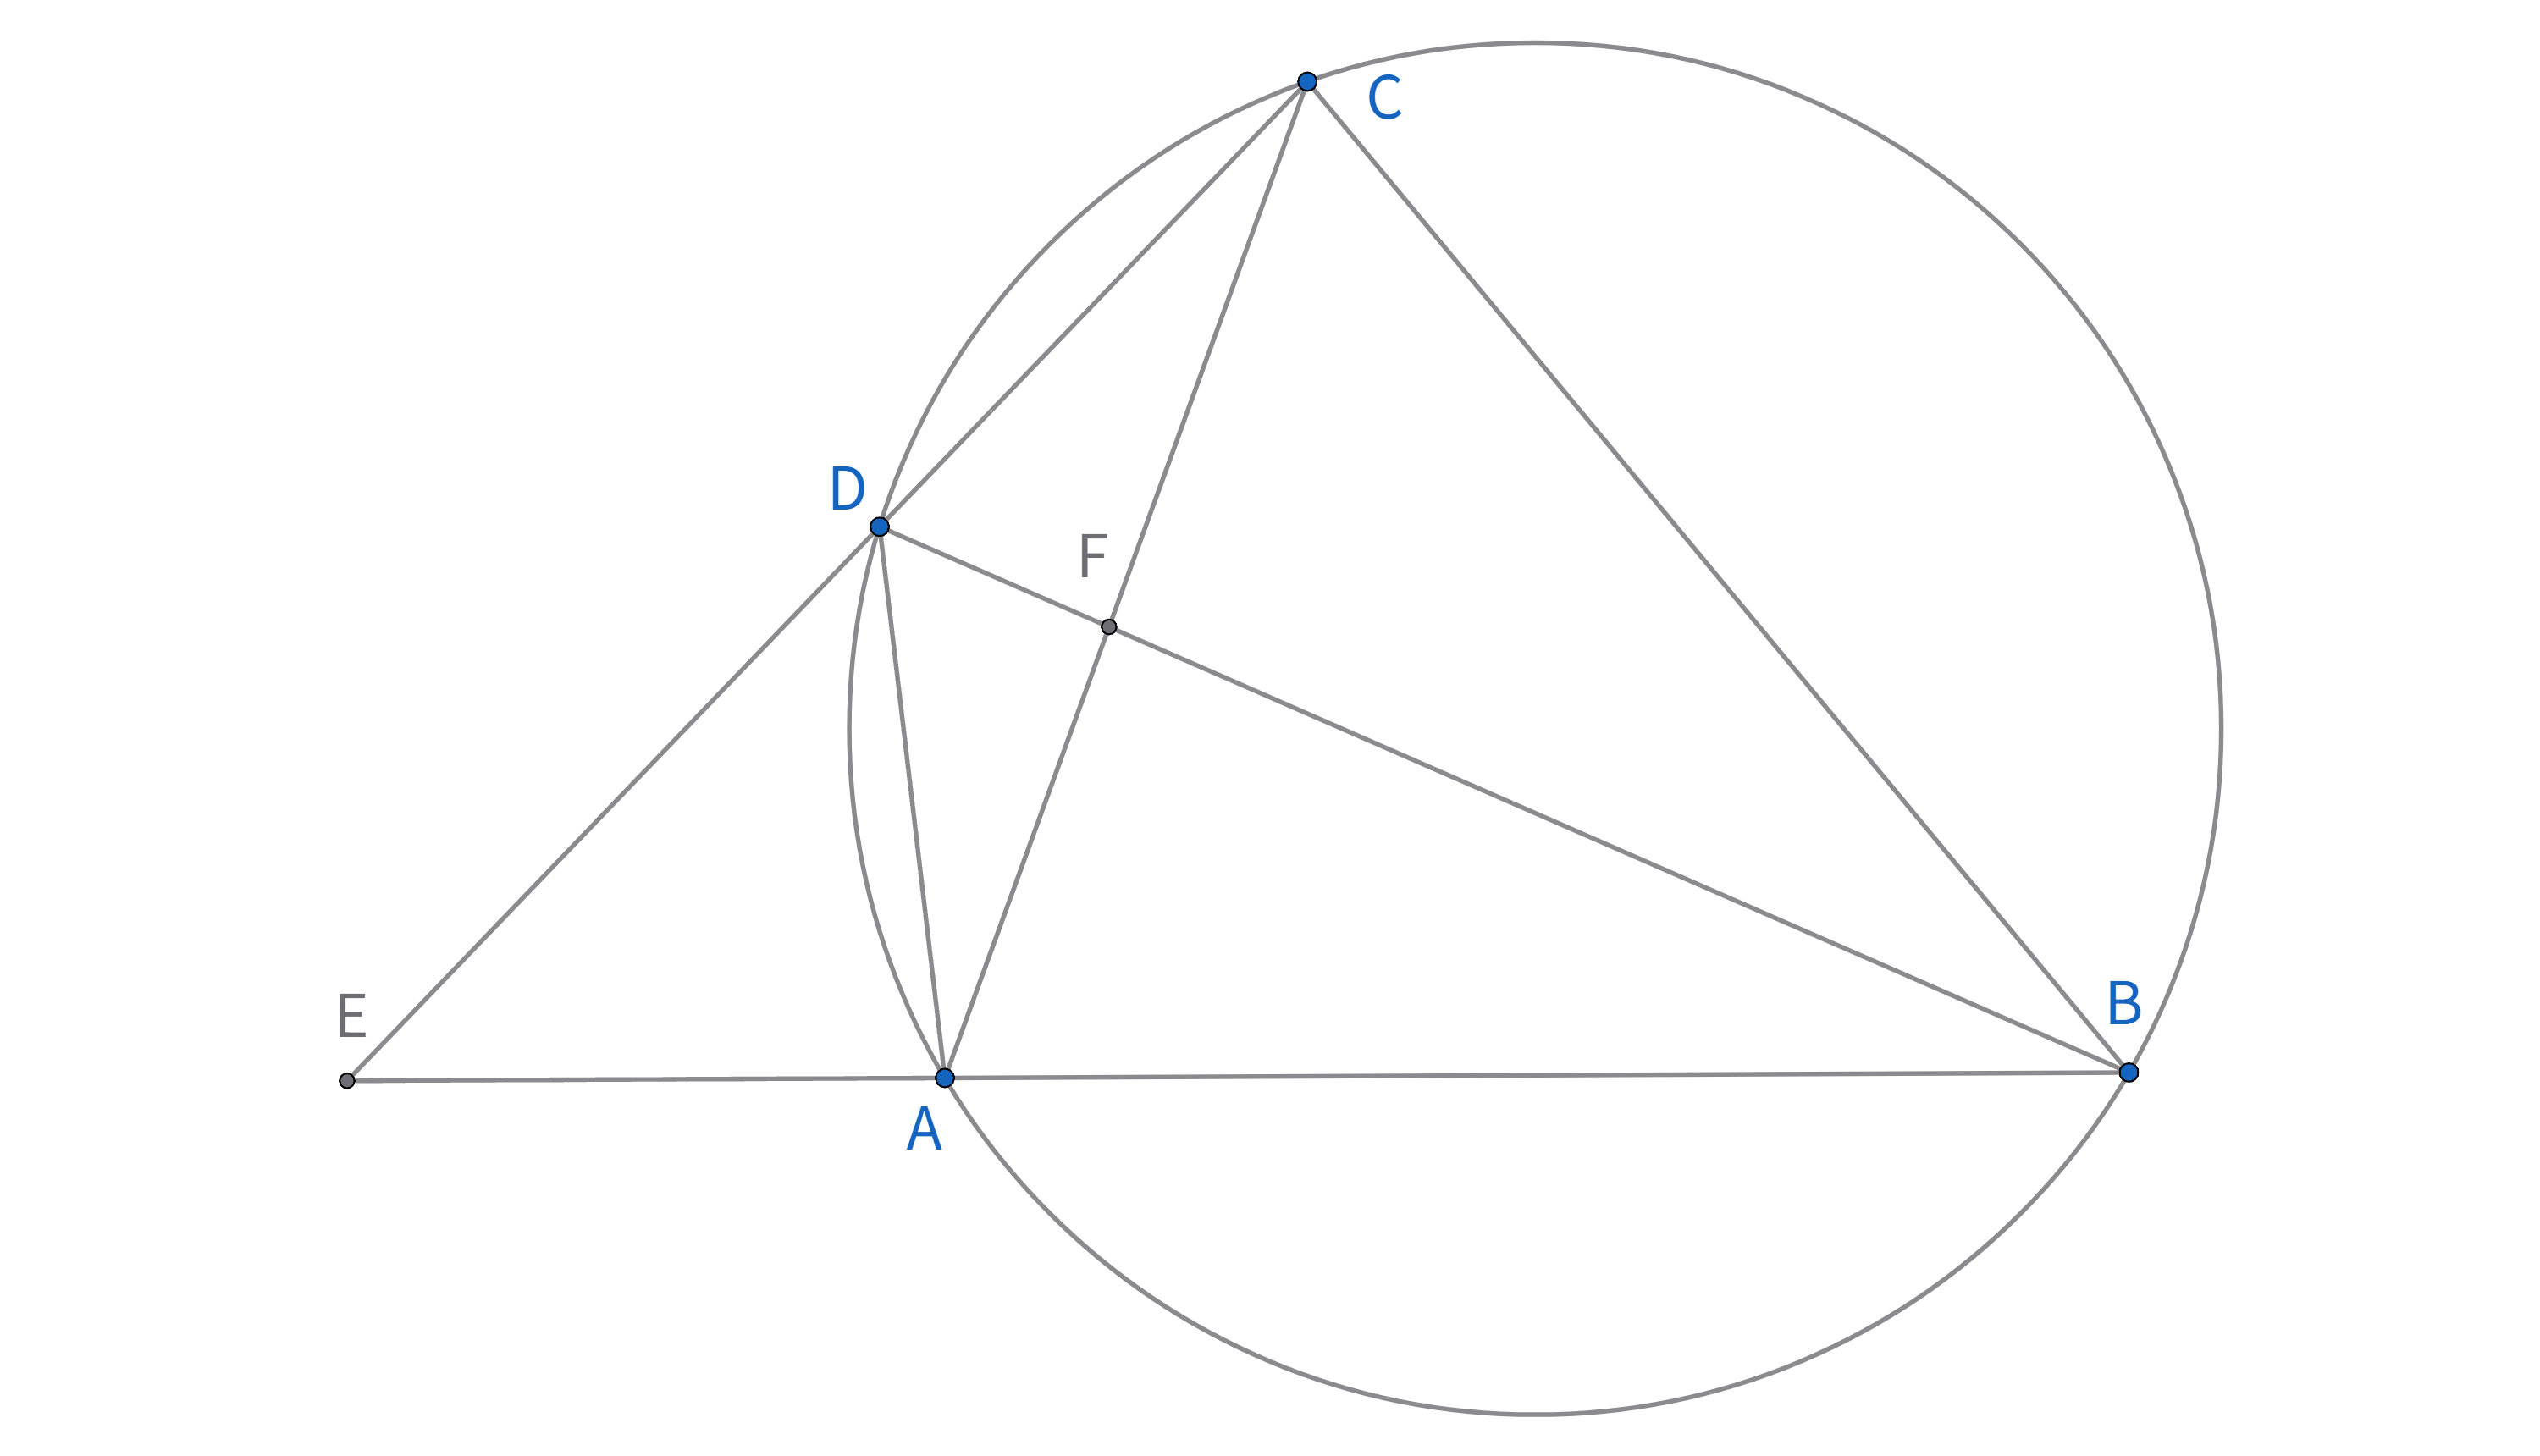
\includegraphics[width=\linewidth]{figures/四点共圆.png}
    % \caption{Caption}
    % \label{fig:enter-label}
\end{figure}




% 蝴蝶定理
\section{蝴蝶定理}
\begin{theorem}
    设M为圆内弦PQ的中点,过M作弦AB和CD。设AD和BC各相交PQ弦于点X和Y,则M是XY的中点。
\end{theorem}

\begin{figure}[H]
    \centering
    \hfill % 添加一些水平间距
    \begin{minipage}[t]{0.45\textwidth}
    \centering
    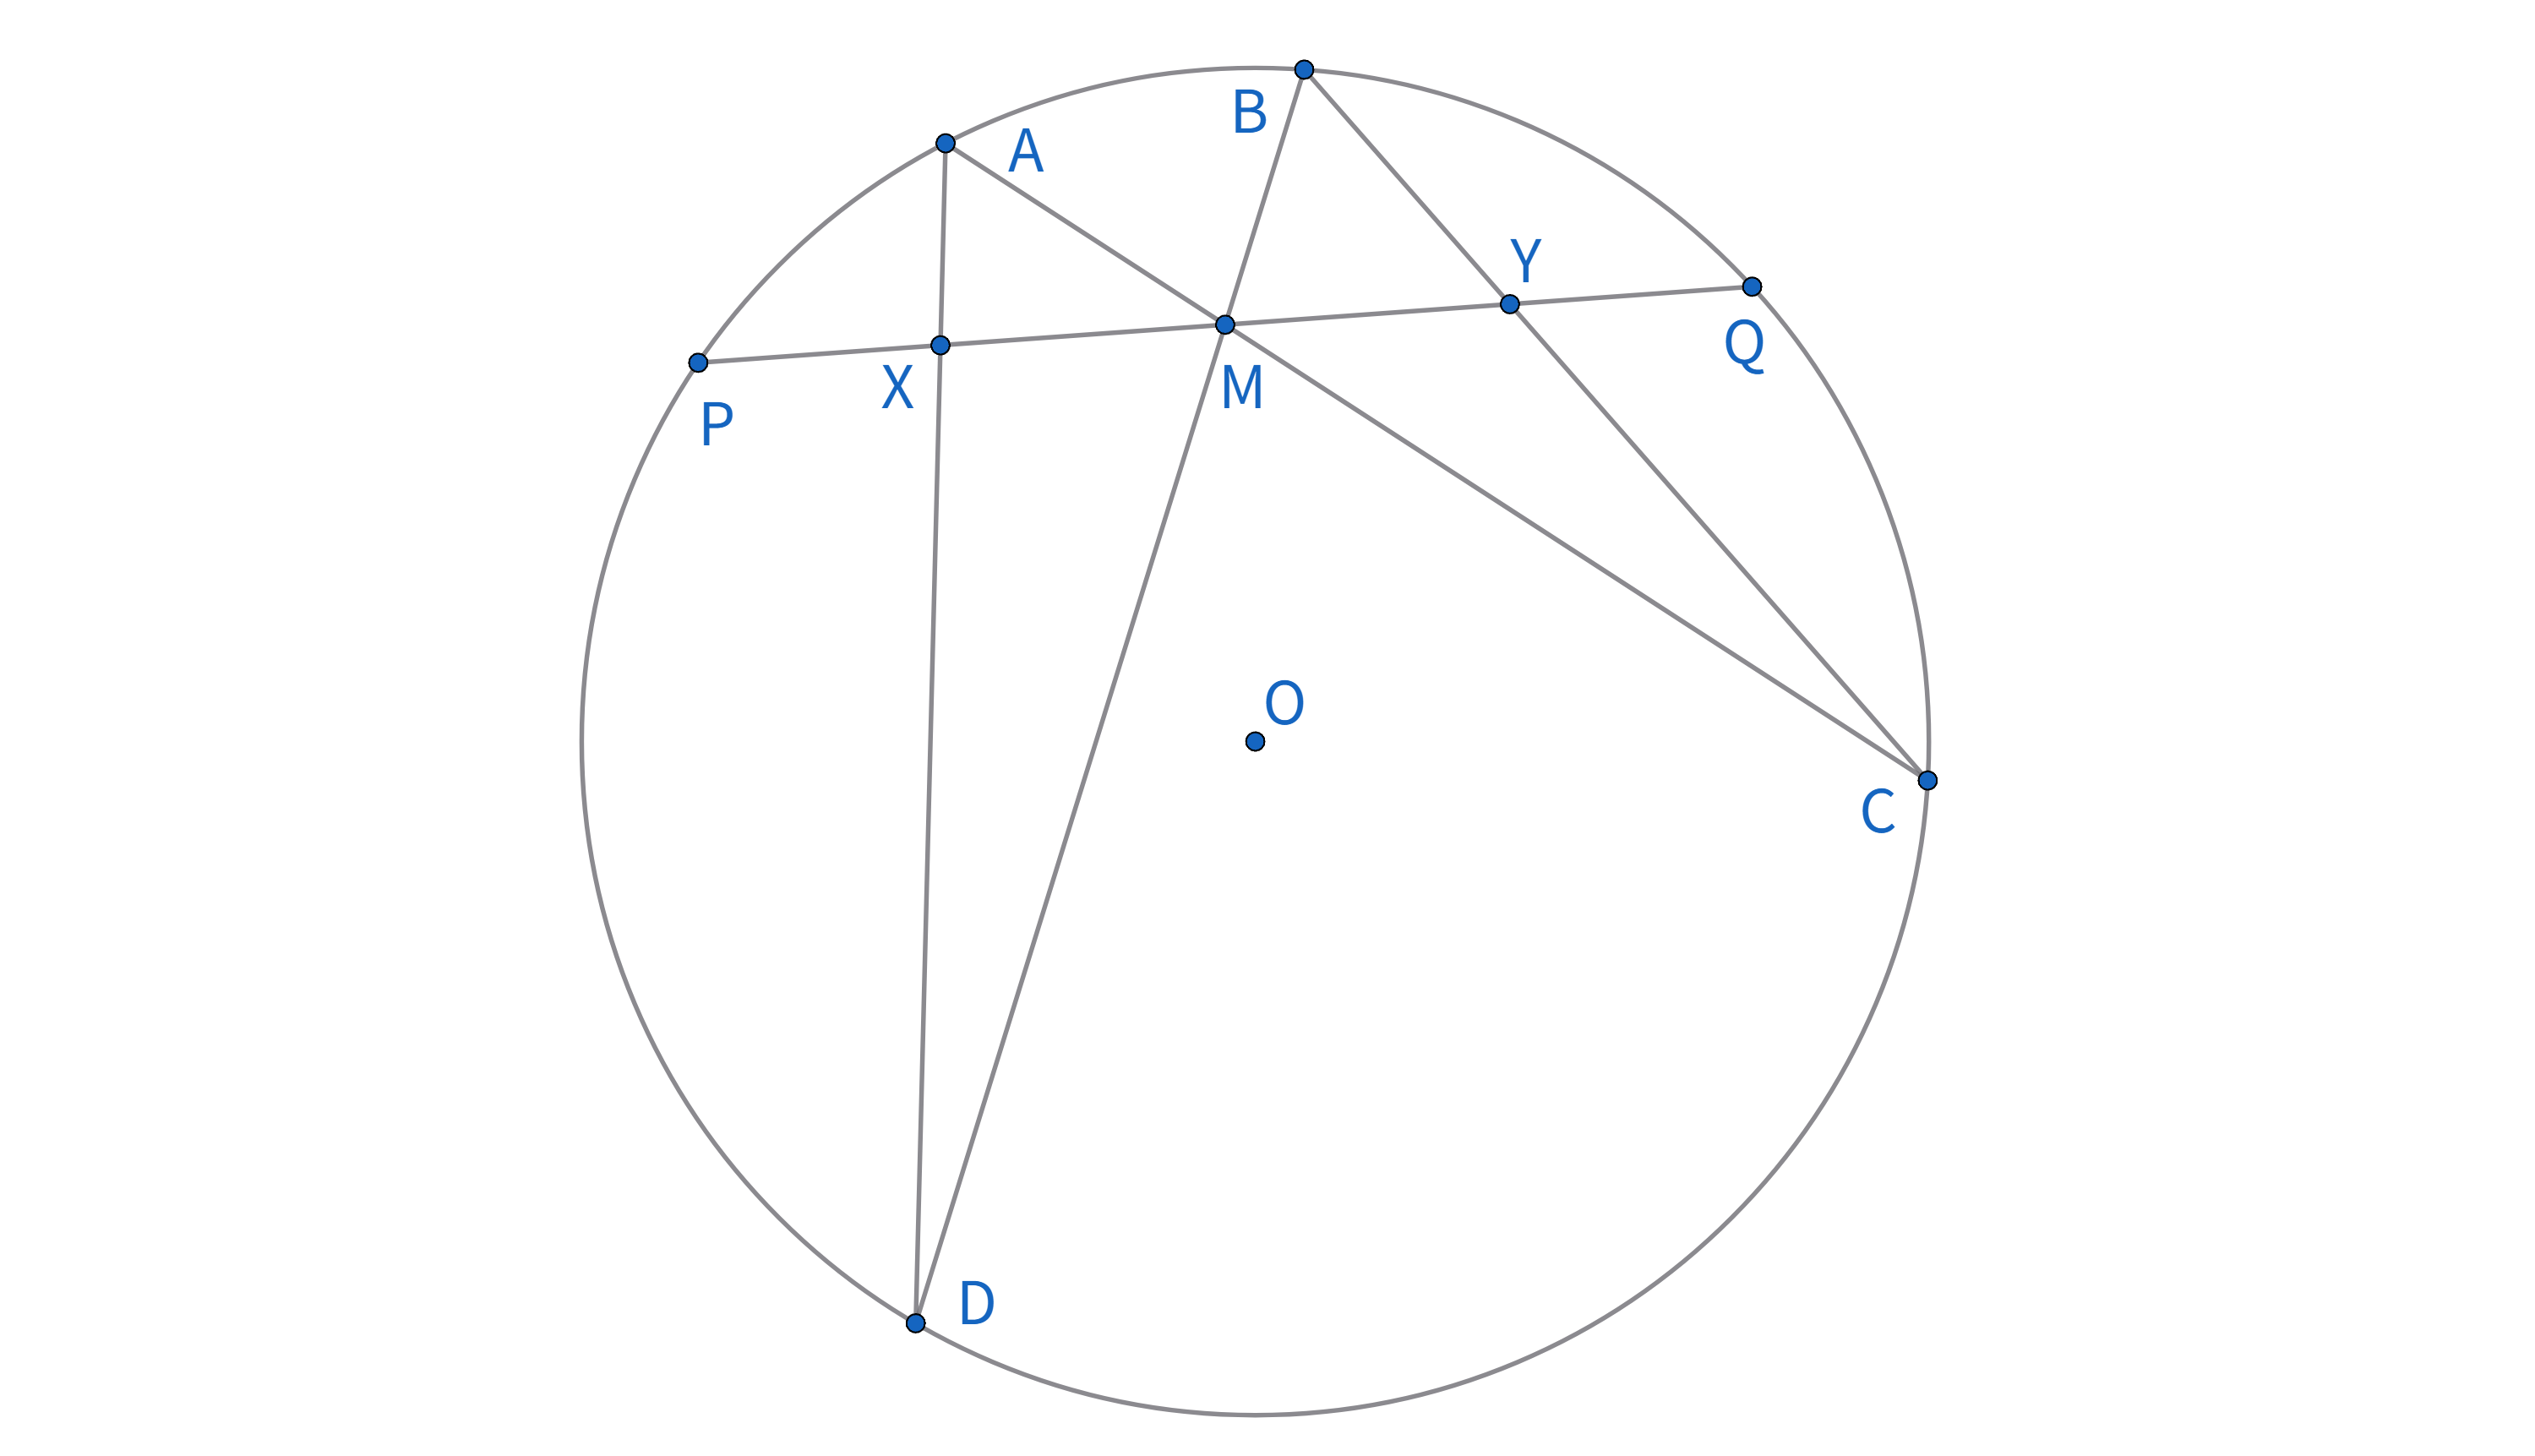
\includegraphics[width=\linewidth]{figures/蝴蝶定理.png}
    \end{minipage}
    \hfill % 添加一些水平间距
    \begin{minipage}[t]{0.45\textwidth}
    \centering
    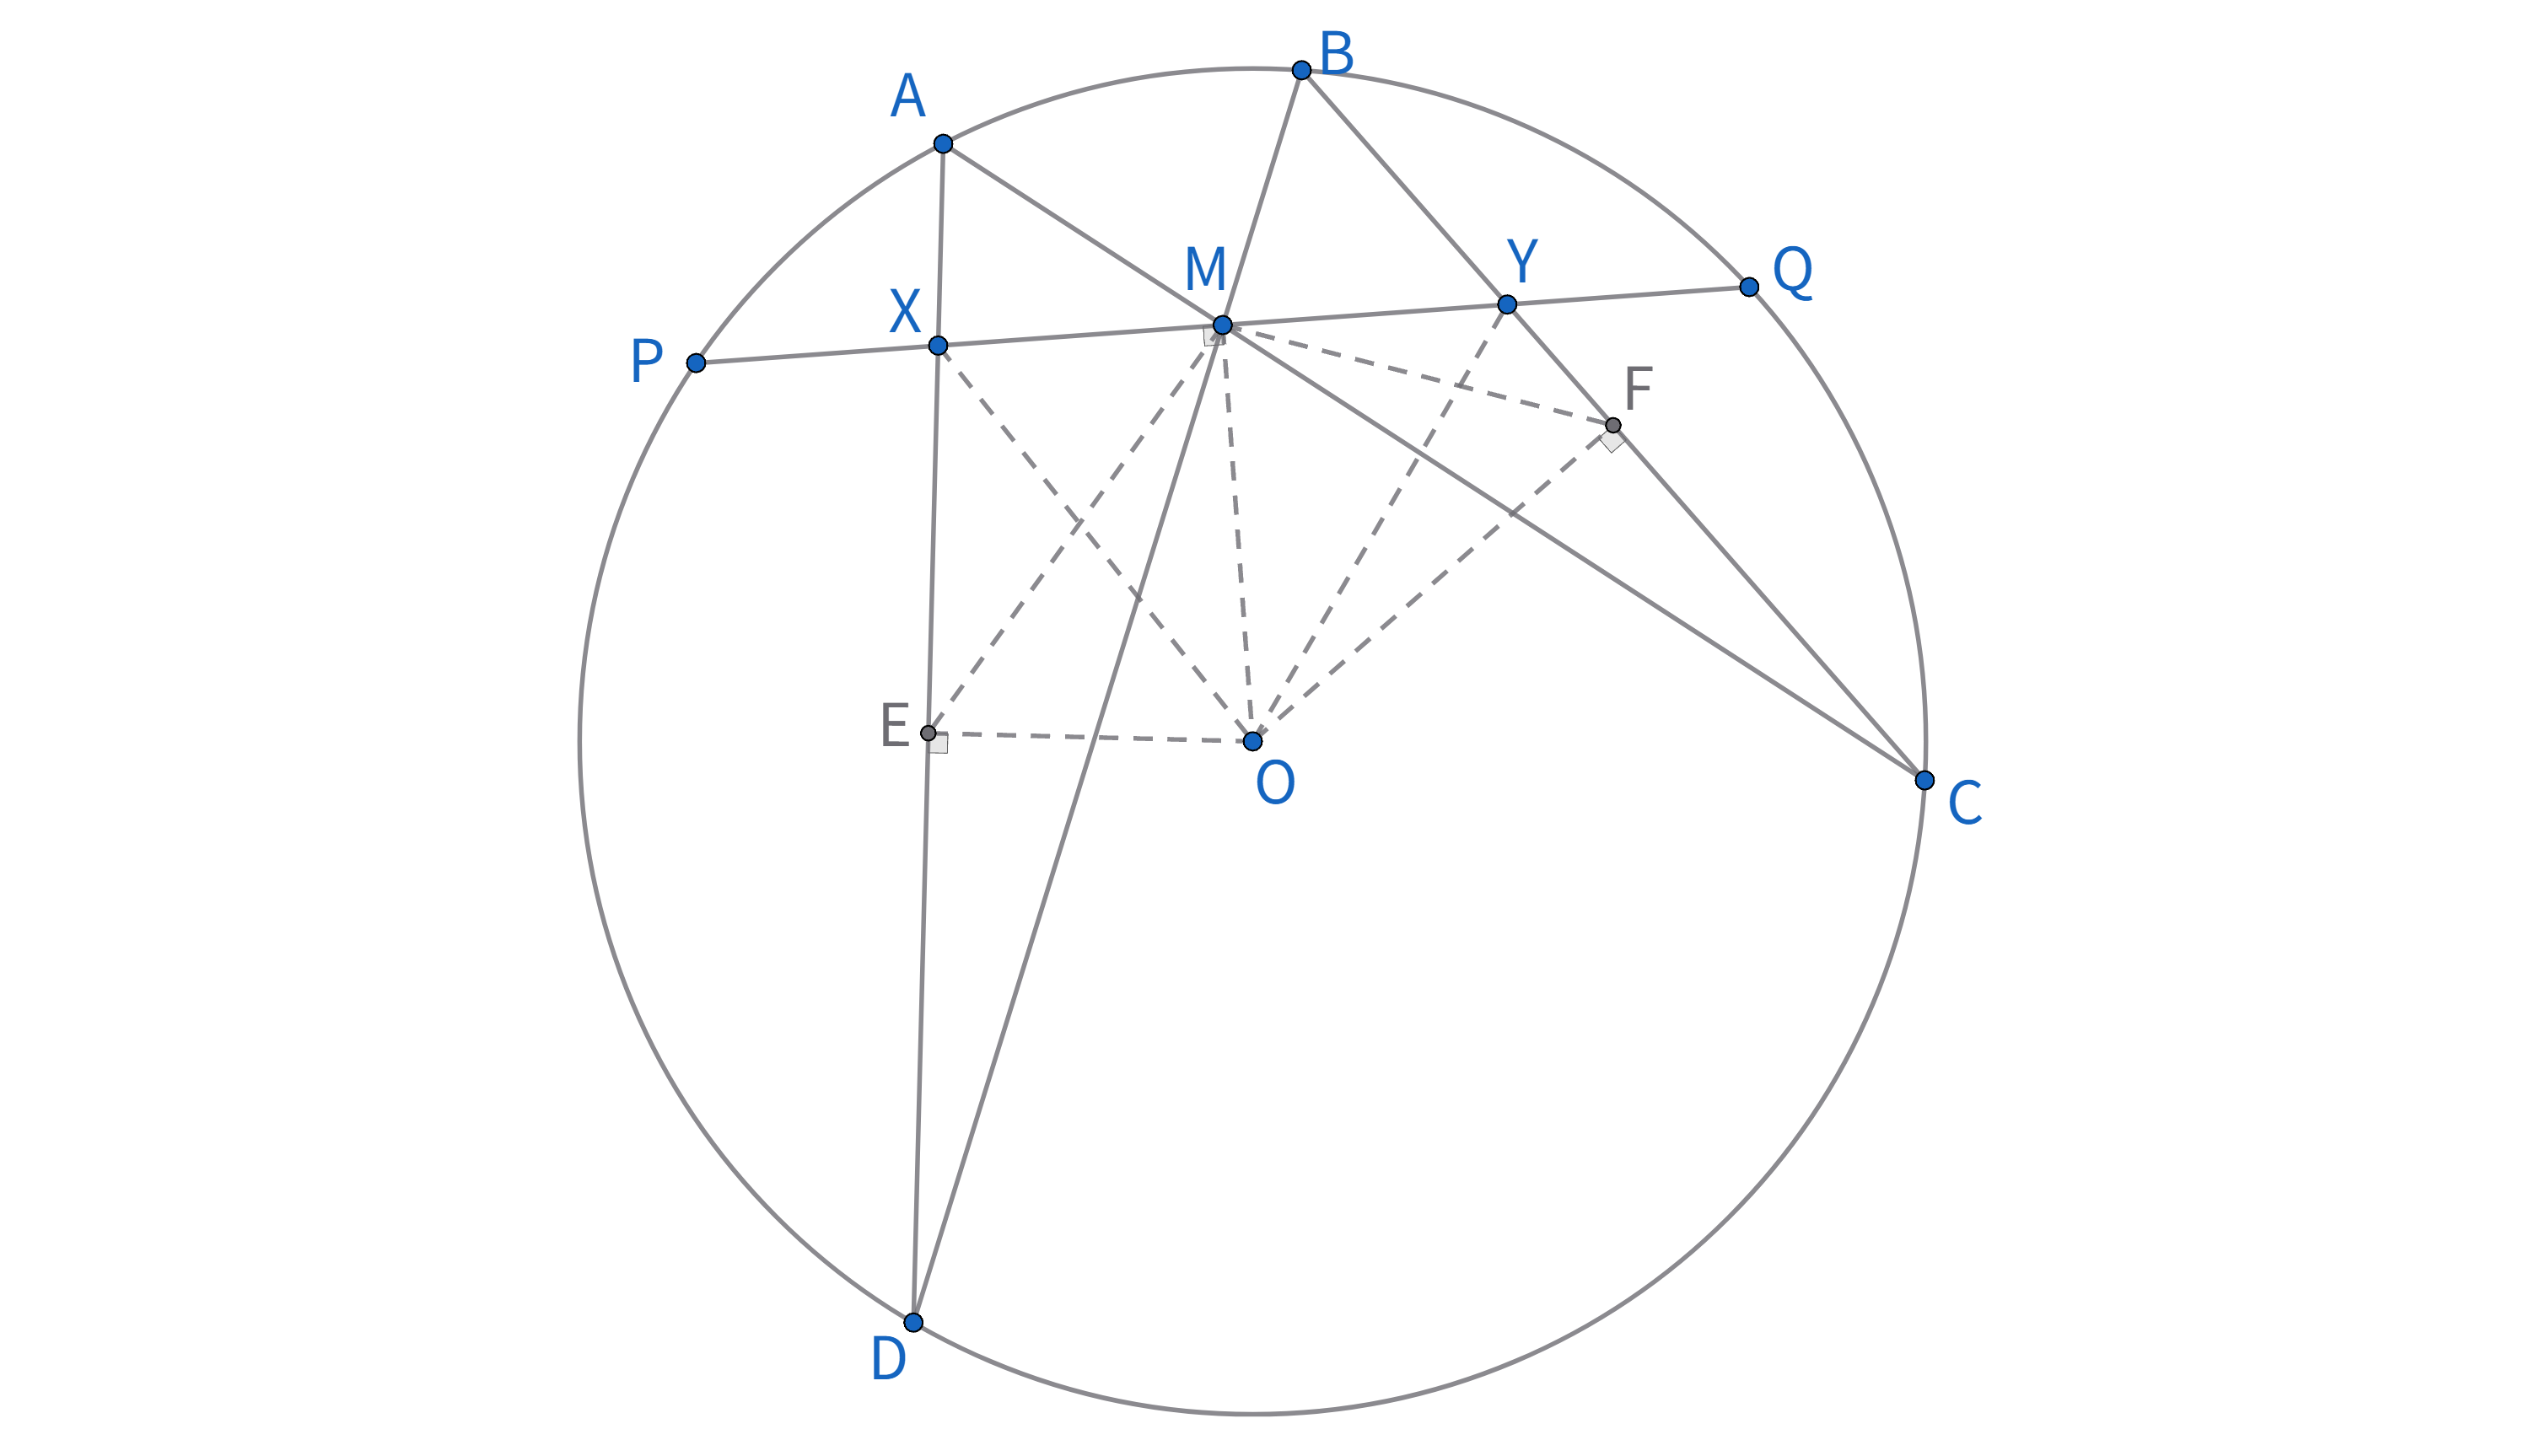
\includegraphics[width=\linewidth]{figures/蝴蝶定理辅助线.png}
    \end{minipage}
\end{figure}



\section{托勒密(Ptolemy)定理}
\begin{theorem}
    圆的内接四边形对角线乘积等于两组对边乘积之和。
    $$AC \cdot BD = AB \cdot CD + BC \cdot AD.$$
\end{theorem}
\begin{figure}[H]
    \centering
    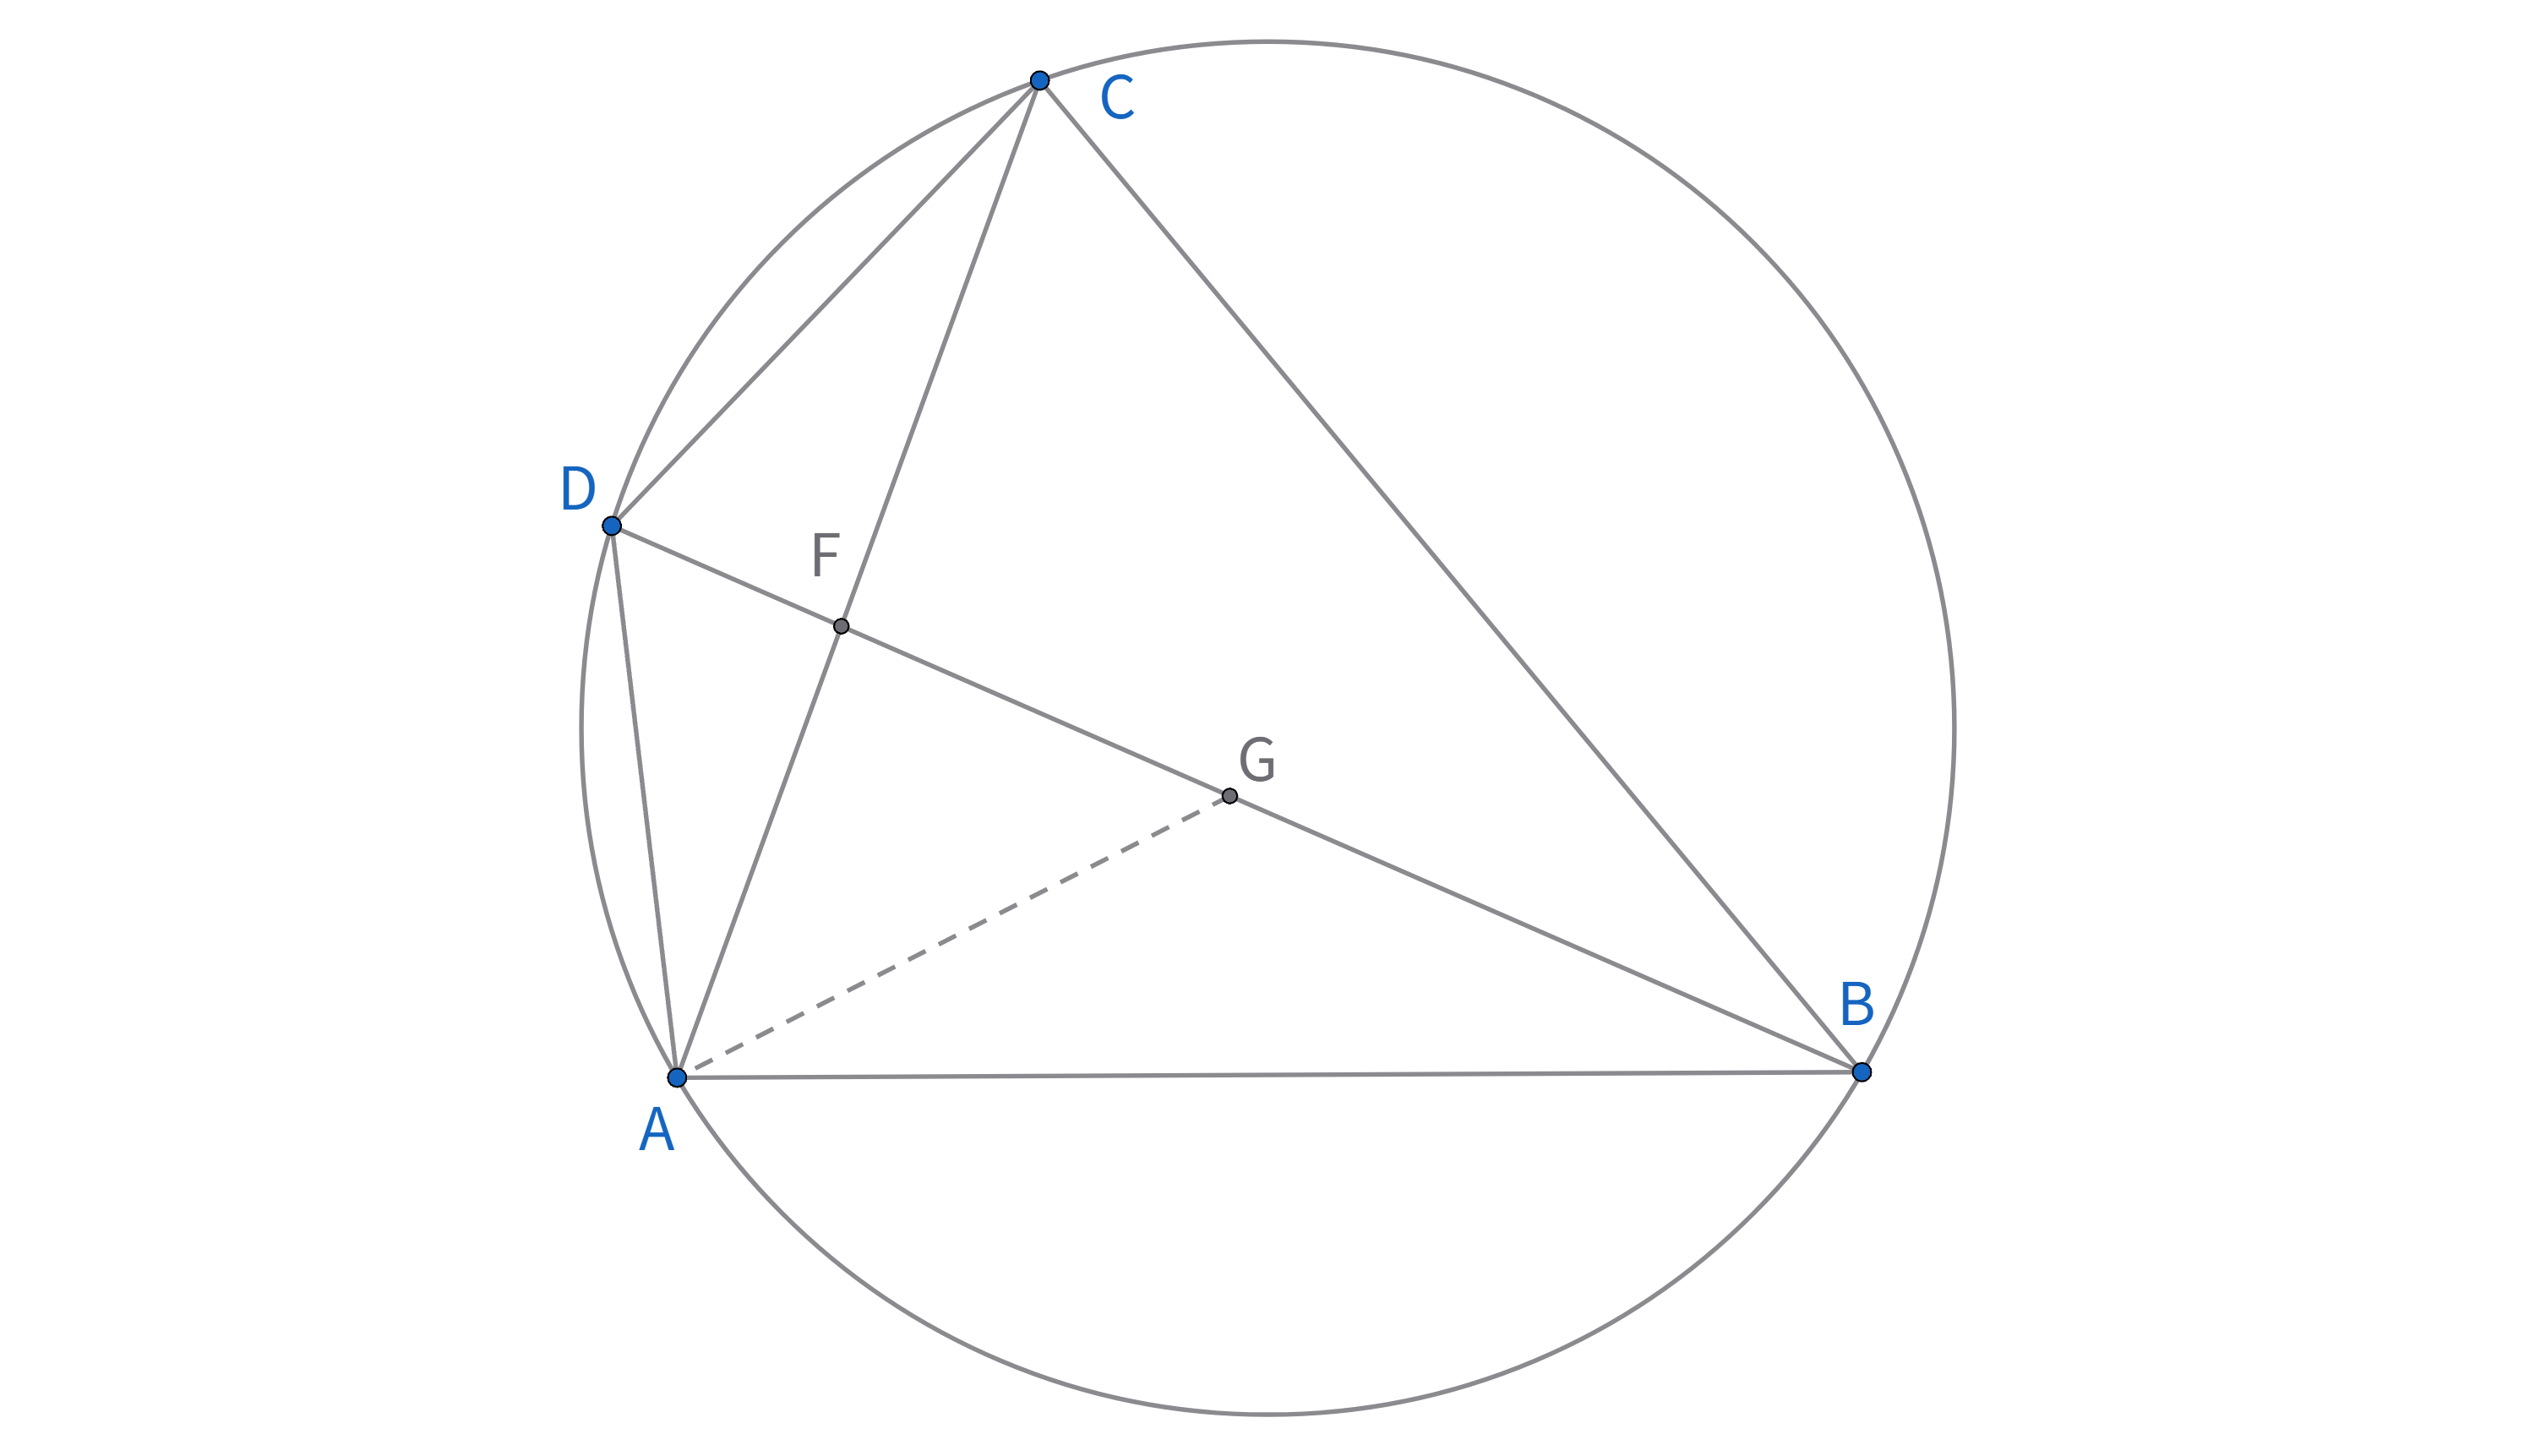
\includegraphics[width=0.7\linewidth]{figures/托勒密定理.png}
    \caption{托勒密定理}
\end{figure}


\section{密克点} 